\documentclass{article}

\usepackage{amssymb}
\usepackage{amsmath}
\usepackage{amsthm}
\usepackage{bm}
\usepackage{graphicx}
\usepackage{hyperref}

\title{CLS Pre-doc Summer School 2017\\NLU with TensorFlow }
\author{Florian Schmidt, Yannic Kilcher\\\small florian.schmidt@inf.ethz.ch, yannic.kilcher@inf.ethz.ch}
\date{July 3, 2017\\\normalsize ETH Zurich, Data Analytics Lab}

\begin{document}
\maketitle
In this exercise we will tackle \textit{binary sentiment classification}, first using convolutional neural networks (CNNs), later using recurrent neural networks (RNNs) . Traditionally this is a supervised learning task. However, since hand-labeled data is a scarce resource, one often resorts to a weakly supervised setting \cite{kim2014convolutional}. Our training data was generated by considering :-) and :-( smileys as a weak learning signal for sentiment. So strictly speaking, our task is to predict which of the two smileys has been removed.

\section*{Exercise 1 - CNN Sentiment Classification}


\paragraph{Dataset} We provide a large set of training tweets, one tweet per line. The dataset is available at
\begin{center}
\url{https://polybox.ethz.ch/index.php/s/5hOF0DqGAmdUYSd}.
\end{center} 
All tweets have been pre-processed so that all words (tokens) are lower-cased and separated by a single whitespace. Tweets in \texttt{*.pos.txt} files are positive tweets and those in \texttt{*.neg.txt} files are negative ones. We suggest you start testing your code with the smaller files and move to the \texttt{full} files once you are confident that your model is doing what it should.\\



\paragraph{Model}
Two dimensional filter operations have a long history in signal and image processing. Accordingly, CNNs have their origin in computer vision. Since the advent of neural word-embeddings \cite{turian2010} \cite{mikolovSCCD13} \cite{glove} it has become common to treat words as $d$-dimensional vectors and sentences as concatenated vectors (e.g. as $d\times n$ matrices for a sentence of length $n$). Given this two-dimensional real-valued sentence representation, we can now apply the same convolutional techniques as in computer vision. Take a look at  \cite{kim2014convolutional} \cite{severyn15} \cite{deriuLLSMCHJ17} if you are interested in the model we implement here.\\

Our model is shown in Figure~\ref{fig:cnn}. The first layer embeds words into low-dimensional vectors. The next layer performs convolutions over the embedded word vectors using multiple filter sizes. For example, sliding over 3, 4 or 5 words at a time. Next, we max-pool the result of the convolutional layer into a long feature vector, add dropout regularization, and classify the result using a softmax layer. We will use only one channel for the convolution.

\begin{figure}[ht]
\centering
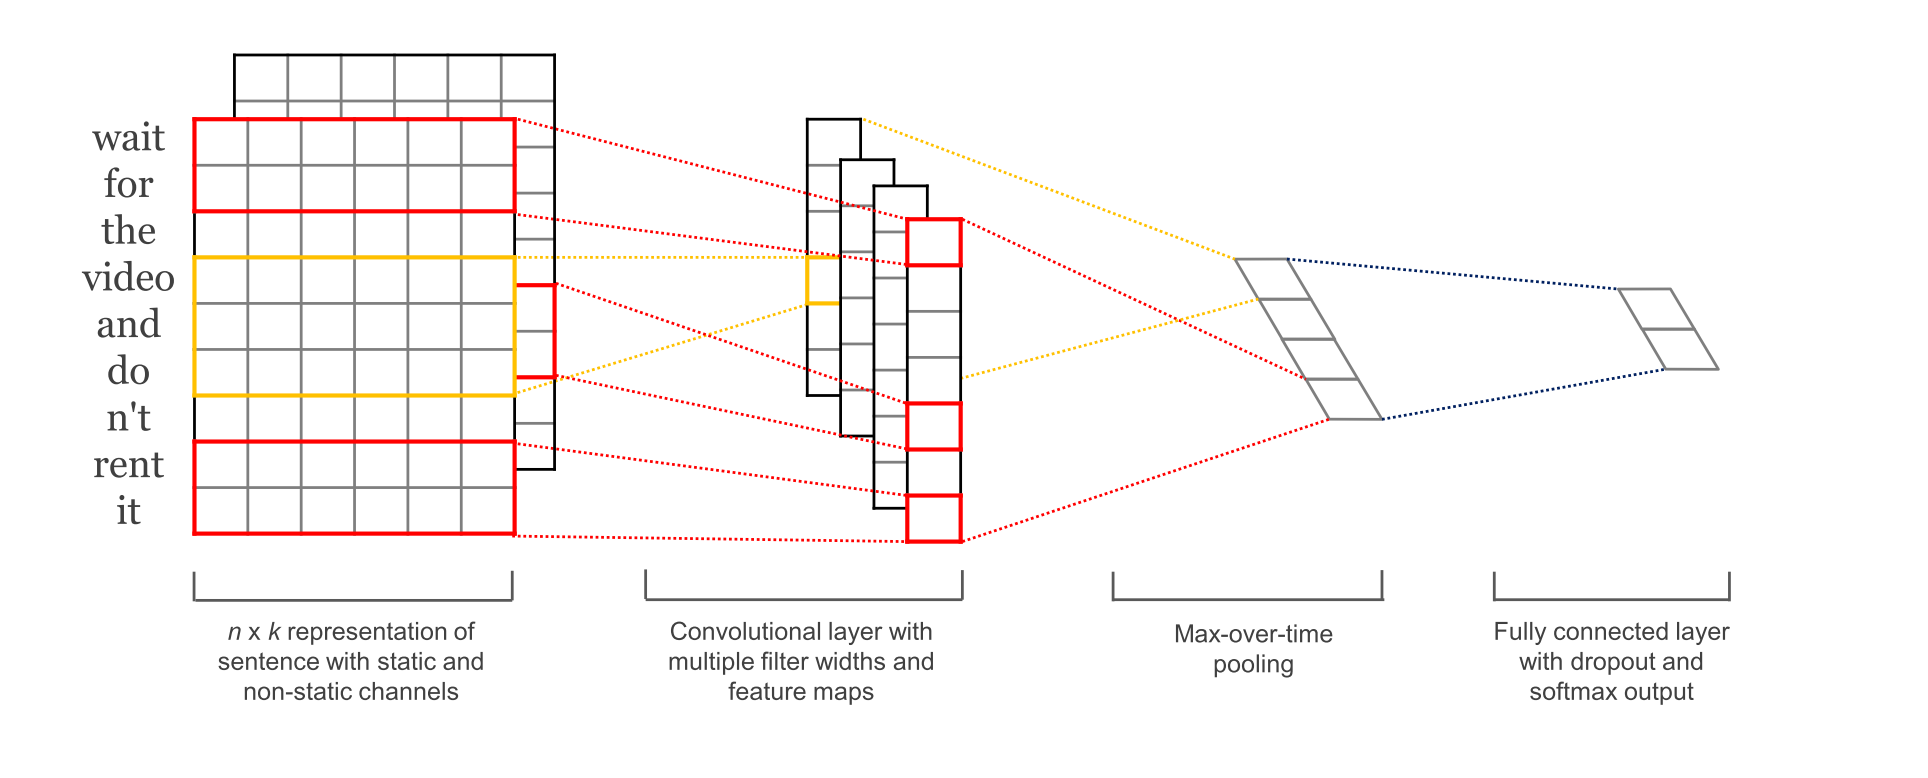
\includegraphics[width=0.95\textwidth]{images/cnn.png}
\caption{CNN model for sentiment classification (from \cite{kim2014convolutional})}
\label{fig:cnn}
\end{figure}

\paragraph{Getting started} To get you up to speed quickly, we provide you with a code skeleton located in the \texttt{code} folder of the repository. This code loads the data, feeds it into a skeleton tensorflow model and performs a training loop.  To be precise:
\begin{itemize}
\item The code loads the data, shuffles it and splits it into a training and a (1000 tweets) dev set.
\item Then we pad the tweets with a $<$PAD$>$ token to the length of the longest tweet. This allows us to use mini-batches since all the tweets will now be of the same size.
\item We convert each word from every tweet to the corresponding index of the word in the vocabulary. Essentially, each tweet becomes a vector of integers.
\item 
The first (embedding) layer of the CNN receives as input a batch of tweets in this format, and replaces each index with a word embedding for the particular word.
\item These word embeddings can be randomly initialized, but typically for NLP tasks it is better to set their initial value to some pretrained word embeddings which our code does. Make sure you have gensim installed\footnote{\texttt{pip3 install --user gensim} should be sufficient. Also see \url{https://radimrehurek.com/gensim/install.htm}}. The word pre-trained embeddings are available at \url{https://polybox.ethz.ch/index.php/s/55YodCdz5nVWtEo}.
\item \textbf{Important}: In order to run the code, you need to provide the following program arguments 	
\begin{verbatim}
--training_file_pos /path/to../train_pos.txt
--training_file_neg /path/to../train_neg.txt
--embedding_file /path/to../glove_model.txt
\end{verbatim}
\end{itemize}
\paragraph{Your task}
\begin{enumerate}
	\item Try to understand the code skeleton we provide, in particular take a look at \texttt{train\_step} and \texttt{dev\_step}. This is where data is fed into TF and results are retrieved. What is the difference between the two?
	\item Complete the code for the CNN (in \texttt{text\_cnn.py}). You find all necessary steps and some hints in the comments. If you get stuck, you can take a look at \texttt{text\_cnn\_solution.py}.
	\item Start your program and start tensorboard\footnote{You need to start a separate python process e.g. using \texttt{python -m tensorflow.tensorboard --logdir /path/to/the/out/directory} in a terminal. Now you can access \url{http://localhost:6006} in your browser. If the page does not render properly, use Google's Chrome browser. See \url{https://www.tensorflow.org/get_started/summaries_and_tensorboard} for a detailed description of tensorboard.}. If your code is correct, the accuracy on the dev set should go from 0.5 to something between 0.7 and 0.8 within about 2000 steps.
	\item Perform the following experiments:
	\begin{enumerate}
		\item Investigate the impact of the pre-trained wordembeddings by commenting out the indicated line in \texttt{train\_cnn.py}. Train with the same parameters and compare in tensorboard.
		\item Change the parametrization of the convolution, e.g.\ the number of filters and their width. What gives you the best results? When is the model saturated?
		\item Investigate the impact of the regularization by setting it to some very large and very small value. What do you observe?
\end{enumerate}	 
\end{enumerate}


\section*{Exercise 4 - RNN Sentiment Classification}

As shown in the slides, RNNs can solve the same sentiment classification task by iteratively building up a summary of the sentence. With your CNN implementation at hand, it's actually only a few lines of codes to implement the RNN.

\paragraph{The Model}
A recursive neural network, recursively computes a sequence of hidden states $h_1,h_2\dots\in\mathbb R^d$. Often this computation also depends on some input $x_1,x_2,\dots\in\mathbb R^{d'}$ and we can write
\begin{align*}
	f_\theta&: \mathbb R^d \times \mathbb R^{d'} \rightarrow \mathbb R^d\\
	h_t&=f_\theta(h_{t-1},x_t)
\end{align*}
where $\theta$ is the parametrization of the network that we want to learn. In this case we can say that an RNN maps a sequence of inputs to a sequence of outputs while maintaining a state $h_t$. In our case the inputs will be words of a sentence and the state will be our sentence summary. At the end of the sentence, this summary should provide a fixed-size representation of the sentence that we can use to predict the sentiment. Just like the CNN max-pooling representation. Figure \ref{fig:rnnArchitecture} shows the general RNN architecture. 
\begin{figure}[ht]
	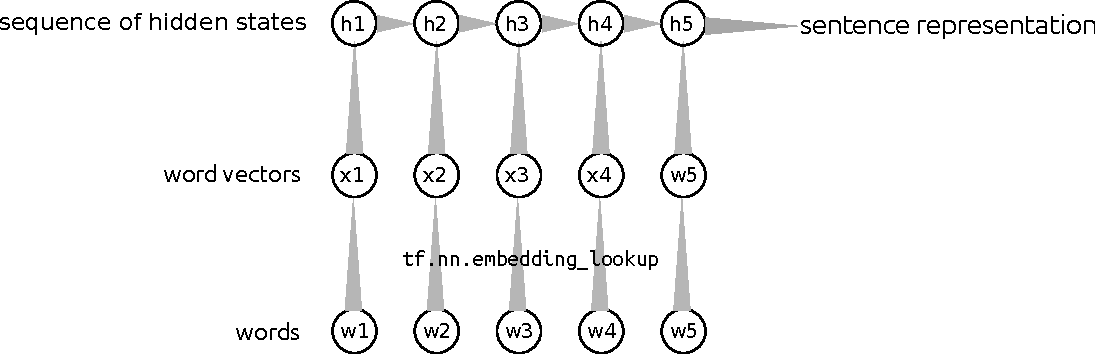
\includegraphics[scale=0.6]{images/rnn.pdf}
	\caption{Abstract RNN architecture}
	\label{fig:rnnArchitecture}
\end{figure}


\paragraph{Your task}
Create a new class \texttt{TextRNN} by copying the content of \texttt{TextCNN} from \texttt{text\_cnn\_solution.py}. Remove all the code between the \texttt{embedding} and the \texttt{dropout} scope. In between these two, we will define a new vector sentence-representation, now using an RNN instead of a CNN. Change the name of this representation from \texttt{self.h\_pool\_flat} to something more appropriate and adapt the size of the fully connected layer after the dropout accordingly. Also, you might want to change the constructor arguments of \texttt{TextRNN} to reflect the hyperparameters of the RNN.

\begin{enumerate}
	\item Define the recurrent computation using the cell classes\footnote{\url{https://www.tensorflow.org/api\_docs/python/tf/nn/rnn\_cell}} of tensorflow. Use \texttt{ tf.nn.rnn\_cell.BasicRNNCell} for a start. The number of hidden units is a hyper-parameter. Try 64 as a start.
	
	\item Use \texttt{tf.nn.static\_rnn} to define your RNN given the cell from above. The returned final state is your new sentence representation. This function expects a \emph{python list} of tensors as input, so you might want to take a look at \texttt{tf.unstack}.
	\item Run the model: 
	\begin{enumerate}
	\item Open the graph in tensorboard (graph tab at the top). You should see a nested graphical representation of your network with boxes that can be expanded. Try to identify the RNN computation. Where is the chain of cells? 
	\item Use an LSTM cell\footnote{See \url{http://colah.github.io/posts/2015-08-Understanding-LSTMs/} or the original paper\cite{hochreiter1997} for an explanation of the recurrent computation.} instead of the RNN cell. Compare the performance of the two by running with the same hyper-parameters.
	\item Open the graph of the LSTM network in the tensorflow. Expand the box of one of the cells. Do you recognize the computation of the gates? Do you see the trick they use to compute all the gates at once?
	\item Change the size of the hidden state size. How is performance affected?
	\end{enumerate}
\end{enumerate}


\bibliography{exercise_tf}
\bibliographystyle{alpha}
\end{document}
